% Options for packages loaded elsewhere
\PassOptionsToPackage{unicode}{hyperref}
\PassOptionsToPackage{hyphens}{url}
%
\documentclass[
]{article}
\usepackage{amsmath,amssymb}
\usepackage{lmodern}
\usepackage{ifxetex,ifluatex}
\ifnum 0\ifxetex 1\fi\ifluatex 1\fi=0 % if pdftex
  \usepackage[T1]{fontenc}
  \usepackage[utf8]{inputenc}
  \usepackage{textcomp} % provide euro and other symbols
\else % if luatex or xetex
  \usepackage{unicode-math}
  \defaultfontfeatures{Scale=MatchLowercase}
  \defaultfontfeatures[\rmfamily]{Ligatures=TeX,Scale=1}
\fi
% Use upquote if available, for straight quotes in verbatim environments
\IfFileExists{upquote.sty}{\usepackage{upquote}}{}
\IfFileExists{microtype.sty}{% use microtype if available
  \usepackage[]{microtype}
  \UseMicrotypeSet[protrusion]{basicmath} % disable protrusion for tt fonts
}{}
\makeatletter
\@ifundefined{KOMAClassName}{% if non-KOMA class
  \IfFileExists{parskip.sty}{%
    \usepackage{parskip}
  }{% else
    \setlength{\parindent}{0pt}
    \setlength{\parskip}{6pt plus 2pt minus 1pt}}
}{% if KOMA class
  \KOMAoptions{parskip=half}}
\makeatother
\usepackage{xcolor}
\IfFileExists{xurl.sty}{\usepackage{xurl}}{} % add URL line breaks if available
\IfFileExists{bookmark.sty}{\usepackage{bookmark}}{\usepackage{hyperref}}
\hypersetup{
  pdftitle={Community Dectection Assignment},
  pdfauthor={David Terner},
  hidelinks,
  pdfcreator={LaTeX via pandoc}}
\urlstyle{same} % disable monospaced font for URLs
\usepackage[margin=1in]{geometry}
\usepackage{graphicx}
\makeatletter
\def\maxwidth{\ifdim\Gin@nat@width>\linewidth\linewidth\else\Gin@nat@width\fi}
\def\maxheight{\ifdim\Gin@nat@height>\textheight\textheight\else\Gin@nat@height\fi}
\makeatother
% Scale images if necessary, so that they will not overflow the page
% margins by default, and it is still possible to overwrite the defaults
% using explicit options in \includegraphics[width, height, ...]{}
\setkeys{Gin}{width=\maxwidth,height=\maxheight,keepaspectratio}
% Set default figure placement to htbp
\makeatletter
\def\fps@figure{htbp}
\makeatother
\setlength{\emergencystretch}{3em} % prevent overfull lines
\providecommand{\tightlist}{%
  \setlength{\itemsep}{0pt}\setlength{\parskip}{0pt}}
\setcounter{secnumdepth}{-\maxdimen} % remove section numbering
\usepackage{booktabs}
\usepackage{longtable}
\usepackage{array}
\usepackage{multirow}
\usepackage{wrapfig}
\usepackage{float}
\usepackage{colortbl}
\usepackage{pdflscape}
\usepackage{tabu}
\usepackage{threeparttable}
\usepackage{threeparttablex}
\usepackage[normalem]{ulem}
\usepackage{makecell}
\usepackage{xcolor}
\ifluatex
  \usepackage{selnolig}  % disable illegal ligatures
\fi

\title{Community Dectection Assignment}
\author{David Terner}
\date{02/27/2022}

\begin{document}
\maketitle

I decided to use R and Rmarkdown to complete this assignment because I
wanted to experiment with systematically changing the resolution
parameter (for the Louvain community detection method). By contrast,
Gephi makes it difficult to complete the same experiment.

\hypertarget{which-resolution-to-use}{%
\subsubsection{Which resolution to use?}\label{which-resolution-to-use}}

According to the \texttt{football.txt} file, college team/node values
correspond to team conferences.

\begin{tabular}{l|l}
\hline
value & conference\\
\hline
0 & Atlantic Coast\\
\hline
1 & Big East\\
\hline
2 & Big Ten\\
\hline
3 & Big Twelve\\
\hline
4 & Conference USA\\
\hline
5 & Independents\\
\hline
6 & Mid-American\\
\hline
7 & Mountain West\\
\hline
8 & Pacific Ten\\
\hline
9 & Southeastern\\
\hline
10 & Sun Belt\\
\hline
11 & Western Athletic\\
\hline
\end{tabular}

I pick a resolution value \(t^*\) such that: (i) the number of
communities equals the number of conferences, namely 12; and, (ii) each
conference has, on average, the majority of its teams belong to to the
same community. I operationalize this second requirement by first
computing the share of top community (largest number of occurrences) per
conference group, second determining the median share, and finally
adjusting the resolution parameter such that this median share is
maximized. Denote this median share value as the \emph{sameness rate}.

I search over a grid of 100 values of the resolution parameter from 0.01
to 1.01 by 0.01 increments.

The figure below presents the \emph{sameness rate}- measured by the blue
line and left vertical axis- and the number of communities-measured by
the black line and right vertical axis-in the same plot. The red dashed
lines correspond to the smallest/largest resolution values that yield 12
communities. Based on the small blue spike that is intersected by the
red dashed boundary line, I choose \(t^*=0.32\) as the resolution value.

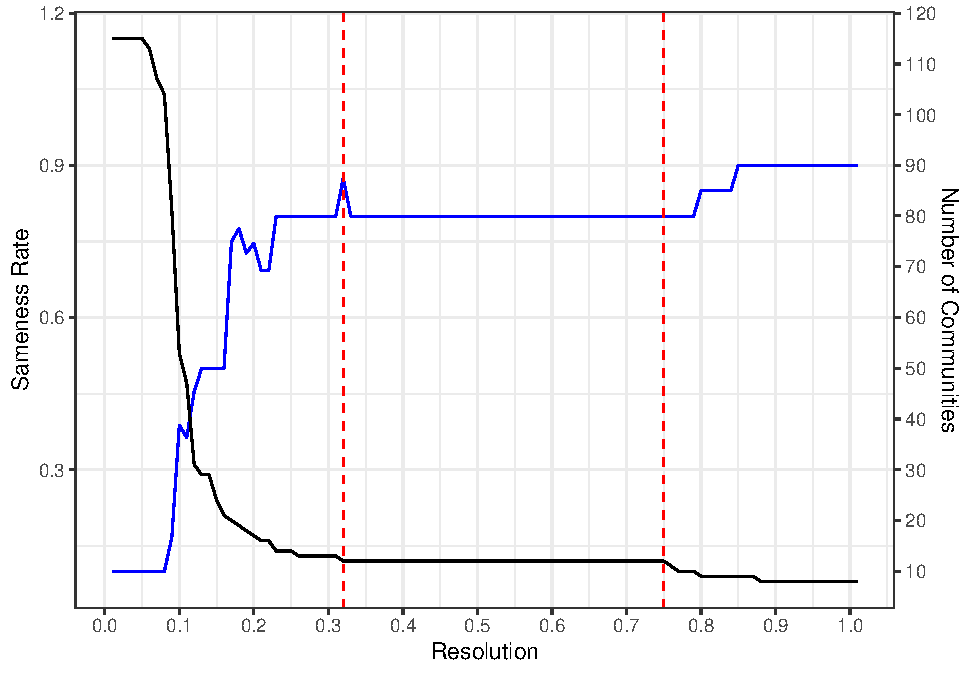
\includegraphics{communities_writeup_files/figure-latex/unnamed-chunk-6-1.pdf}

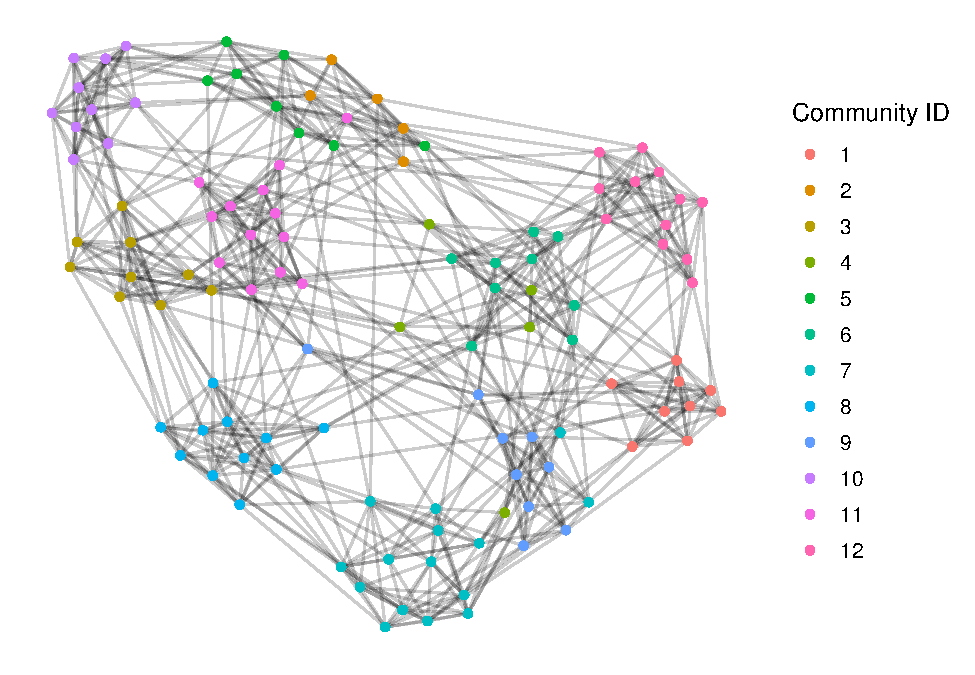
\includegraphics{communities_writeup_files/figure-latex/unnamed-chunk-8-1.pdf}

\begin{tabular}{l|r}
\hline
Conference & Top Community Share\\
\hline
Atlantic Coast & 1.00\\
\hline
Big Ten & 1.00\\
\hline
Big Twelve & 1.00\\
\hline
Mid-American & 1.00\\
\hline
Mountain West & 1.00\\
\hline
Pacific Ten & 1.00\\
\hline
Southeastern & 1.00\\
\hline
Conference USA & 0.90\\
\hline
Big East & 0.88\\
\hline
Western Athletic & 0.80\\
\hline
Sun Belt & 0.43\\
\hline
Independents & 0.40\\
\hline
\end{tabular}

Using the Forced Atlas layout, the college football league does appear
to have some community structure to it. Using the \(t^*=0.32\)
resolution does a pretty good job matching communities to conferences: 7
out of 12 conferences consist of exactly one community. On the lower
end, there is less of tight fit especially with the ``Independents''
conference. This shouldn't come as a shock given which schools belong to
the ``Independents'' conference; Central Florida, Connecticut, Navy,
Notre Dame, and Utah State are clearly a diverse group of programs with
little in common save football conference membership. By contrast, the
``Big 10'' conference is exclusive to the MidWest.

\hypertarget{how-are-betweenness-centrality-and-community-structure-related}{%
\subsection{How are betweenness centrality and community structure
related?}\label{how-are-betweenness-centrality-and-community-structure-related}}

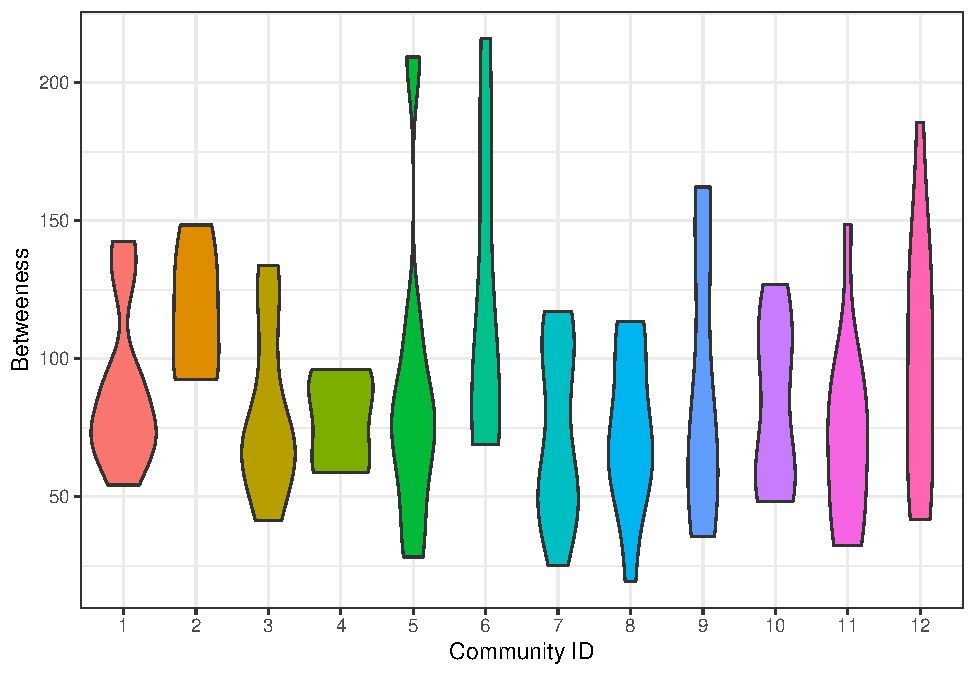
\includegraphics{communities_writeup_files/figure-latex/unnamed-chunk-10-1.pdf}
Based on the above figure, there doesn't appear to be a strong
relationship between between ``betweeness'' and ``modularity''. Nodes
within a community can all have betweeness scores that relatively close
to one another; see communities 4+5. However for other communities, such
as 6 or 12, there's substantial betweeness variation.

\end{document}
